\section{Problem 3: Debye Solid}


\subsection{Analytical Methodology}

The Debye heat capacity is given by Simon \cite[page 13]{Simon2013} as
\begin{align*}
    C(T) &= N_\text{atom}k_B\frac{(k_B T)^3}{(\hbar \omega_\text{Debye})^3}\frac{12\pi^4}{5}
\end{align*}

\subsection{Results}

\subsubsection{Numerical and Analytical Heat Capacity}
%
The numerical and analytical Debye heat capacities are shown in Fig. (\ref{debye_numerical_and_analytical_heat_capacities}). Across the temperature range 0.1 to 200 K, the numerical heat capacities show strong agreement with their analytical counterparts, but with decreasing agreement closer to 200 K.
\begin{figure}[h]
    \centering
    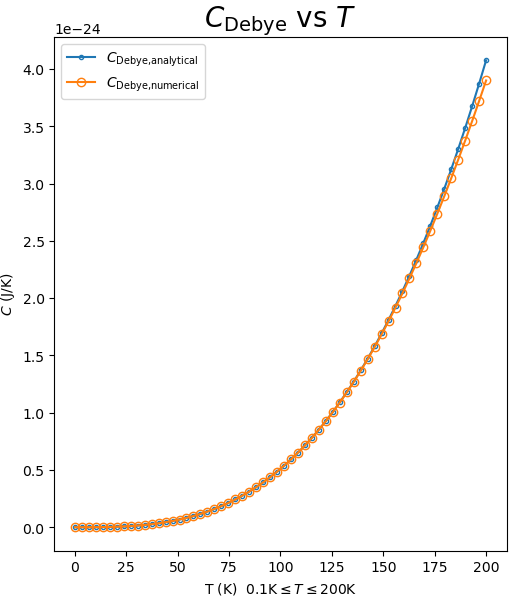
\includegraphics[width=9cm]{debye_numerical_and_analytical_heat_capacities.png}
    \caption{Numerical and Analytical Debye Heat Capacity vs Temperature}
    \label{debye_numerical_and_analytical_heat_capacities}
\end{figure}
\begin{table}[h]
\begin{center}
    \footnotesize
    \begin{tabular}{|c|c|c|}
        \hline
        \textbf{System Parameter} & \textbf{Value} & \textbf{Notes} \\ \hline
        No. of Atom(s) & 1 & - \\ \hline
        Debye Frequency & 2.422$\times 10^{14}$ s$^{-1}$ & for Diamond, from Simon \cite[page 13]{Simon2013} \\ \hline
        Finite Difference Magnitude ($\Delta T$) & 0.001 K & arbitrary \\ \hline
    \end{tabular}
\end{center}
\caption{System Parameters for Fig. (\ref{debye_numerical_and_analytical_heat_capacities})}
\label{system_parameters_for_Debye_heat_capacity}
\end{table}

\newpage
\subsubsection{Einstein and Debye Heat Capacities Compared}
%
The previously-obtained numerical and analytical Einstein and Debye heat capacities are shown together in Fig. (\ref{einstein_and_debye_heat_capacities}). As before, the numerical and analytical Einstein heat capacities show strong agreement with each other across the temperature range 0.1 K to 2000 K. The numerical Debye heat capacities are greater than the Einstein heat capacities at lower temperatures, and are less than the Einstein heat capacities at higher temperatures, with the transition point being located around 300 K. The analytical Debye heat capacities begin to deviate significantly from the other three at around 250 K.
\begin{figure}[h]
    \centering
    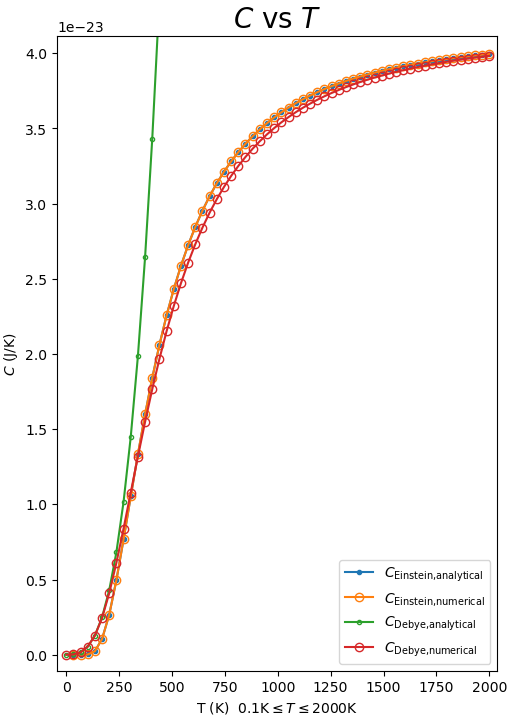
\includegraphics[width=10cm]{einstein_and_debye_heat_capacities.png}
    \caption{Einstein and Debye Heat Capacity vs Temperature}
    \label{einstein_and_debye_heat_capacities}
\end{figure}



\subsection{Discussion}

The Debye model is an improvement on the Einstein model in that the former takes into account the fact that one atom may take on many different vibrational frequencies (normal modes) and not just one, the Einstein frequency.